%\section{Project Logic}
\chapter{Project Logic}
\label{chap:logic}
%\pagenumbering{arabic}

The reasoning in this work started by considering the characters of a problem that is recognizable as Farm parallel pattern.
Then the study moved to considering how a GPU works, main architectural characteristics and its data parallel nature.
Next we had to think how to "merge" two such different behaviors, in order to reach reasonable performances \footnote{About that see sect ****** for more clarifications}, i.e. almost competitive with a classic data parallel problem.
Finally, once the main idea behind the development was clear, we had to make some tunings.
All of these steps will be shown in detail in next sections.

\section{Streaming Parallelism: Farm pattern}
Stream parallel patterns describe problems exploiting parallelism among computations relative to
different, independent data items appearing on the program input stream.
Each independent computation end with the delivery of one single item on the program output stream.\\
We focused on farm pattern, modeling embarrassingly parallel stream parallelism. 
For example, consider the correspondent skeleton:\\
\texttt{let rec farm f =\\
	function\\
	EmptyStream -> EmptyStream\\
	| Stream(x,y) -> Stream((f x),(farm f y));;\\
	}
	
whose type is\\
\( farm :: (\alpha \rightarrow \beta) \rightarrow \alpha stream \rightarrow \beta stream \)\\

\textit{The parallel semantics, associated to the higher order functions, states that the computation of any items appearing on the input stream is performed in parallel}\\

In the farm case, according to the parallel semantics a number of parallel agents computing function f onto input data items equal to the number of items appearing onto the input stream could be used. This is not realistic, however, for two different reasons:

\begin{enumerate}
	\item items in the stream do not exist all at the same time. A stream is not a vector.
	Items of the stream may appear at different times. Actually, when we talk of consecutive items \(x_{i}\) and \(x_{i+1}\) of the stream we refer to items appearing onto the stream at times \(t_{i}\) and \(t_{i+1}\) with \(t_{i} < t_{i+1}\). As a consequence, it makes no sense to have a distinct parallel agent for all the items of the input stream, as at any given time only a fraction of the input stream will be available.
	
	\item  if we use an agent to compute item \(x_{k}\), presumably the computation will end at some
	time \(t_{k}\). If item \(x_{j}\) appears onto the input stream at a time \(t_{j} < t_{k}\) this same agent
	can be used to compute item \(x_{j}\) rather than picking up a new agent. \\
\end{enumerate}


This is why the parallelism degree of a task farm is a critical parameter: a small parallelism degree doesn't exploit all the parallelism available (thus limiting the speedup), while a large parallelism degree may lead to inefficiencies as part of the parallel agents will be probably idle most of time \cite{spm}.\\

%In some skeleton frameworks, therefore, the parallelism degree is given as a parameter of
%the skeleton. The task farm skeleton is therefore defined as an high order function having
%(also) an integer as a parameter. This parameter represent their intended parallelism degree
%of the implementation of the skeleton. 
However it has no effect on the “function” computed by the skeleton. It has only effect on the “parallel semantics” metadata.
%A task farm skeleton with a parallelism degree parameter may therefore be defined with
%the high order function
%let rec farm f n:int =
%function
%EmptyStream -> EmptyStream
%| Stream(x,y) -> Stream((f x),(farm f y));;
%whose type is now
%f arm :: (α → β) → int → α stream → β stream
%with the parallel semantics defined as follows:
%the computation of consecutive items of the input stream is performed in parallel on
%n parallel agents.
%These non functional parameters of skeletons generated quite a huge debate within the skeleton community. 
%On the one side, as skeletons pretend to abstract all the aspects related
%to parallelism exploitation, non functional parameters such as the parallelism degree should
%not be left under application programmer responsibility. Rather, they should be properly
%handled by the skeleton implementation, possibly being computed using some performance
%model of the skeleton (see Chap. 5). On the other side, such parameters can be used by
%expert programmers to express the fact they want to use exactly that amount of resources.
%As an example, they may want to experiment different parallelism degrees according to the
%type of the execution constrains of the applications. If the computation of the results is
%not urgent, smaller parallelism degrees may be required, whereas, in case of very urgent
%computations, higher parallelism degrees may be asked through non functional parameters.
%Consistently with the idea a skeleton is a programming abstraction hiding all the details
%related to parallelism exploitation pattern implementation, we agree on the idea that the
%better choice is to leave to the skeleton implementation the management of all the non
%functional skeleton parameters. In case the programmer is allowed to provide such kind of
%parameters, they will be only taken as loose requirements on the execution of the skeleton:
%the implementation of the skeleton will try to accommodate user requests, but in case
%the implementation could figure out the requests are not reasonable or that better choices
%could be made, these better choices will be actually taken and the user will be consequently
%informed.


%3.2.1
%Stream modelling
%An alternative way of defining stream parallel algorithmic skeletons assumes pipeline and
%farm just operate on a global input stream of data to produce a global stream of results. In
%this case, we may define pipelines and farms with much simpler higher order functions that
%do not operate on streams, actually, and then use these functions as parameters of another
%higher order function implementing stream parallelism. In this case, the pipeline skeleton
%will basically correspond to functional composition:
%let pipeline f g =
%function x -> (g (f x));;
%while task farm skeleton corresponds to identity:
%let farm f =
%function x -> (f x);;
%The higher order function taking care of exploiting parallelism can then be defined as follows:
%let rec streamer f x =
%match x with
%EmptyStream -> EmptyStream
%| Stream (v,s) -> Stream ((f v), (streamer f s));;
%such that, to define the filter/recognize program defined in Sec. 3.2 we can now write:
%let main =
%streamer (pipeline filter recognize);;
%Clearly, the parallel semantics associated to skeletons changes in this case, with respect
%to the parallel semantics we had when pipeline and farms actually processed streams. A
%parallel semantics is only associated to the streamer function as:
%the processing of independent input stream data items is performed in parallel
%whereas pipeline and farm have do not have associated any kind of parallel semantics.
%This way of modelling stream parallelism corresponds to the idea of structuring all stream
%parallel applications as farms 51 with more coarse grain computations as functional param-
%eter.
%Again, consider the filter/recognize example. Let’s suppose that the recognize phase is
%much more computationally expensive with respect to the filter phase. Using the explicit
%stream handling versions of pipeline and farm skeletons, we would write the program as
%let main =
%pipeline (filter) (farm recognize);;
%51 recall the parallel semantics previously given for the farm and look at the analogies in between the streamer
%function and the former definition of the farm higher order function58
%ALGORITHMIC SKELETONS
%Recalling the parallel semantics of these skeletons we can easily understand that given a
%stream with data items x 1 , . . . , x m (with x i appearing on the stream after x i−k for any k)
%the computations of
%recognize(y i ) recognize(y i+k )
%(being y i = f ilter(x i )) happen in parallel, as well as the computations of
%recognize(y i ) f ilter(x i+k )
%If we use the alternative modelling of stream parallelism described in this section, the
%program instead is written as
%let main =
%streamer (pipeline filter recognize);;
%and in this case the only computations happening in parallel are the
%recognize(f ilter(x i )) recognize(f ilter(x i+k ))


%3.3 A SIMPLE SKELETON FRAMEWORK
%Although different programming frameworks based on skeletons have been developed that
%sport each different algorithmic skeletons, a subset of common skeletons may be found in
%most of these frameworks. These common subset contains skeletons from three different
%classes of skeletons: stream parallel skeletons, data parallel skeletons and control parallel
%skeletons.
%3.3.1
%Stream parallel skeletons
%Stream parallel skeletons are those exploiting parallelism among computations relative to
%different, independent data items appearing on the program input stream. Each indepen-
%dent computation end with the delivery of one single item on the program output stream.
%Common stream parallel skeletons are the pipeline and task farm skeletons, whose definition
%in terms of higher order functions and parallel semantics has already been given in Sec. 3.2.
%The pipeline skeleton is typically used to model computations expressed in stages. In
%the general case, a pipeline may have more than two stages. The restriction to two stages
%as given by the definition in Sec. 3.3.4 guarantees strong typing and the ability to define
%pipelines with more than two stages as pipelines of pipelines. Given a stream of input tasks
%x m , . . . , x 1
%the pipeline with stages
%s 1 , . . . , s p
%computes the output stream
%s p (. . . s 2 (s 1 (x m )) . . .), . . . , s p (. . . s 2 (s 1 (x 1 )) . . .)
%The parallel semantics of the pipeline skeleton ensures all the stages will execute in
%parallel. In Chap. 5 we will see that this guarantees that the total time required to compute
%a single task (pipeline latency) is closed to the sum of the times required to compute the
%different stages. Also, it guarantees that the time needed to output a new result is close to
%time spent to compute a task by the longer stage in the pipeline.A SIMPLE SKELETON FRAMEWORK
%59
%The farm skeleton is used to model embarrassingly parallel computations, instead. The
%only functional parameter of a farm is the function f needed to compute the single task.
%Given a stream of input tasks
%x m , . . . , x 1
%the farm with function f computes the output stream
%f (x m ), . . . , f ( x 1 )



We recall that the only functional parameter of a farm is the function \(f\) needed to compute the single task.
Given a stream of input tasks
\begin{center}
	\(x_m , . . . , x_1\)\\
\end{center}
the farm with function \(f\) computes the output stream
\begin{center}
	\(f ( x_m ), . . . , f ( x_1 )\)\\
\end{center}
Its parallel semantics ensures it will process the single task in a time close to the time needed to compute \(f\) sequentially. The time between the delivery of two different task results, instead, can be made close to the time spent to compute f sequentially divided by the number of parallel agents used to execute the farm, i.e. its parallelism degree.
\cite{spm}		


\section{CPU-GPGPU: heterogeneous architecture}
The target of this project was to exploit GPGPUs high parallelism to lighten the CPU from computation intensive problems, in particular associated to the above explained Farm parallel pattern.\\
So we asked ourselves what happens if we wanted to manage such computations on stream's elements in a way such that:
\begin{enumerate}
	\item input stream arrives from host side, being directly generated by CPU or acquired from a remote source;
	
	\item items are sent from host (main memory) to the GPU (global memory);
	
	\item GPU cores apply specific computations on all items of the stream (already available in global memory);
	
	\item finally, computed elements will be copied back to host side. \\

\end{enumerate}

	In this list our main concern is about data transfer, i.e. step 2 and 4. 
	Indeed these phases introduce an overhead per se, but especially in Farm parallel pattern they can be a not negligible bottleneck.\\
	We should not forget that our input is a stream: even if elements are available with a high throughput, they come "one by one".
	So, as we mentioned in the previous section, it's not realistic to have one worker per stream element.
	Furthermore, we surely don't want to transfer from/to GPU one element at time, but in some way we have to keep as much as possible the nature of a Stream parallel patterns.\\
	
	Thus at this point has become necessary for first to find a stratagem, to hide as much as we can data transfer times (both in  \(Host \rightarrow Device\)  and  \(Device \rightarrow Host\)  direction).
	
	\subsection{Overlapping: Data Transfer hiding}
	We introduced in  \hyperref[subs:stream]{Section 2.3.3} CUDA Streams, they can perform an asynchronous memory copy to or from the GPU
	concurrently with kernel execution. 
	Since the machines we worked on have both concurrency on data copy and kernel execution and they have 2 copy engines, we exploited this capability  combined with streams.\\
	In this way we wanted to achieve a situation in which we could hide, as much as it was possible, the time it took for the GPU to execute a kernel and the time it took to transfer data back and forth.\\
	
	As an example see Figure \ref{fig:threeStreams} to understand a simple case with 3 CUDA Streams.
	In that diagram we can see the expected behavior  of three streams, but we can extend our expectations to more than three streams, without forgetting that we can have at most 2 data transfer at the same time (given that we've two copy engines).\\
	
	It's important to point out that overlap amount depends on several factors: on the order in which the commands are issued to each stream, whether or not the device supports overlap of data transfer and kernel execution, concurrent kernel execution, and/or concurrent data transfers. Among those factors the only that can influence in our case is the order in which commands are issued to each stream, given that our GPUs supported all kind of above mentioned concurrencies.

	
	
	
	\begin{figure}
		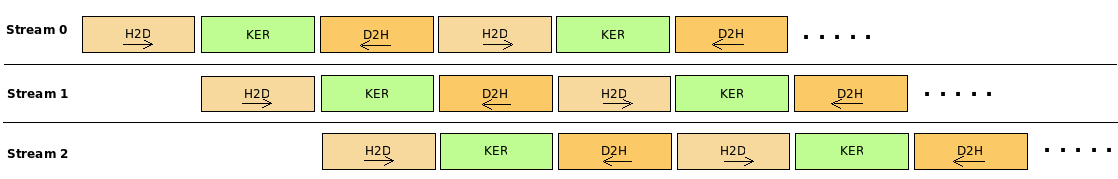
\includegraphics[width=\linewidth]{images/3Streams.png}
		\caption{Ideal behavior for 3 CUDA Streams.}
		\label{fig:threeStreams}
	\end{figure}
	
	Other useful guidelines to improve the potential for concurrent kernel execution:
	\begin{itemize}
		\item All independent operations should be issued before dependent operations,
		\item Synchronization of any kind should be delayed as long as possible.
	\end{itemize}

	For the former, we have that all operations are independent, given the Farm nature. Indeed all stream items and their computation given by workers, are independent.
	For the latter we were careful to avoid introducing host issued operations in-between different streams commands, this should have not introduced 
	\textit{Implicit synchronization}.
	Moreover we avoided all possible \textit{Explicit synchronizations}.
	
	Another important face of overlapping, is that we should try to balance Kernels work in such a way it's sufficient to hide the time spent in data transfers. 
	This said we can have two unfair scenarios:
	\begin{itemize}
		\item data transfers take a small amount of time, while kernels are doing lot of computations;
		\item data transfers take a big amount of time, with respect to time spent in kernel execution.
	\end{itemize}
	
	The former case may arise when we have heavy computations or "irregular kernels".
	By irregular we mean that any flow control instruction (\textbf{if}, \textbf{switch}, \textbf{do}, \textbf{for}, \textbf{while}) can significantly affect the instruction throughput by causing threads of the same warp to diverge; that is, to follow different execution paths. 
	If this happens, the different execution paths must be serialized, increasing the total number of instructions executed for this warp. When all the different execution paths have completed, the threads converge back to the same execution path.	
	So we should avoid different execution paths within the same warp. To obtain best performance in cases where the control flow depends on the thread ID, the controlling condition should be written so as to minimize the number of divergent warps. This is possible because the distribution of the warps across the block is deterministic
	% as mentioned in Section 4.1 of the CUDA C Programming Guide. A trivial example is when the controlling condition depends only on(threadIdx / WSIZE) where WSIZEis the warp size. In this case, no warp diverges because the controlling condition is perfectly aligned with the warps 
	\cite{cudaguide}.\\
	
	The latter case can happen when we move an amount of data at each transfer such that it takes more time than calculations. So in this case the dominant factor will be the data transfer.\\
	
	So about these two scenarios we had to make some assumptions and tunings, that we will see in ********. 
	
	
	
	
	\subsection{Occupancy of GPU cores}
	Once we carried out the stream logic, we had to understand how to try to exploit almost every Streaming Multiprocessor at any given time.
	This means that we wanted to launch as many kernels as they was necessary to reach almost the full \textit{\textbf{Occupancy}}.\\
	Clearly, when we start, we'll have a portion of time, a sort of "warm up" where we'll have first data transfers and few kernels. 
	But as soon as we have enough data transfers and so a lot of kernels.\\
	
	In the reality when we just said lot of kernels we meant, lot of blocks. Let's spend a bit to explain better what Occupancy means.\\

	To maximize utilization the application should be structured in a way that it exposes
	as much parallelism as possible and efficiently maps this parallelism to the various
	components of the system to keep them busy most of the time.
	Here main ways to maximize utilization:
	\begin{enumerate}
			\item \textbf{Application Level}
			At a high level, the application should maximize parallel execution between the host, the
			devices, and the bus connecting the host to the devices, by using asynchronous functions
			calls and streams as described in Asynchronous Concurrent Execution. It should assign
			to each processor the type of work it does best: serial workloads to the host; parallel
			workloads to the devices.
			
			
			\item \textbf{Device Level}
			At a lower level, the application should maximize parallel execution between the multiprocessors of a device.
			Multiple kernels can execute concurrently on a device, so maximum utilization can also be achieved by using streams to enable enough kernels to execute concurrently as described in Asynchronous Concurrent Execution.
			
			
			\item \textbf{Multiprocessor Level}
			At an even lower level, the application should maximize parallel execution between the	various functional units within a multiprocessor.
			In particular, a GPU multiprocessor relies on thread-level parallelism to maximize utilization of its functional units. 
	\end{enumerate}
	
	From the above, it's cleat that occupancy is directly linked to the number of resident warps. At every instruction issue time, a warp scheduler selects a warp that is ready to execute its next instruction, if any, and issues the instruction to the active threads of the warp.\\
	The number of clock cycles it takes for a warp to be ready to execute its next instruction is called the latency, and full utilization is achieved when all warp schedulers always have some instruction to issue for some warp at every clock cycle during that latency period, or in other words,	when latency is completely "hidden". 
	
	The most common reason a warp is not ready to execute its next instruction is that the instruction's input operands are not available yet.
	If all input operands are registers, latency is caused by register dependencies, i.e., some
	of the input operands are written by some previous instruction(s) whose execution has
	not completed yet. In the case of a back-to-back register dependency (i.e., some input
	operand is written by the previous instruction), the latency is equal to the execution
	time of the previous instruction and the warp schedulers must schedule instructions for
	different warps during that time.
	%Execution time varies depending on the instruction, but it is typically about 11 clock cycles for devices of compute capability 3.x, which translates to 44 warps for devices of compute capability 3.x (assuming that warps 	execute instructions with maximum throughput, otherwise fewer warps are needed).
	%This is also assuming enough instruction-level parallelism so that schedulers are always able to issue pairs of instructions for each warp.
	%If some input operand resides in off-chip memory, the latency is much higher: 200 to 400 clock cycles for devices of compute capability 3.x. 
	
	%The number of warps required to keep the warp schedulers busy during such high latency periods depends on the kernel code and its degree of instruction-level parallelism. In general, more warps are required if the ratio of the number of instructions with no off-chip memory operands 	(i.e., arithmetic instructions most of the time) to the number of instructions with off-chip 	memory operands is low (this ratio is commonly called the arithmetic intensity of the program). For example, assume this ratio is 30, also assume the latencies are 300 cycles on devices of compute capability 3.x. Then about 40 warps are required for devices of compute capability 3.x (with the same assumptions as in the previous paragraph).
	Another reason a warp is not ready to execute its next instruction is that it is waiting at some memory fence (Memory Fence Functions) or synchronization point. A synchronization point can force the multiprocessor to idle as	more and more warps wait for other warps in the same block to complete execution of instructions.\\
	Having multiple resident blocks per multiprocessor can help reduce idling in this case, as warps from different blocks do not	need to wait for each other at synchronization points.
	The number of blocks and warps residing on each multiprocessor for a given kernel call depends on the execution configuration of the call (grid and block dimensions), the memory resources of the multiprocessor, and the resource requirements of the kernel as described in Hardware Multithreading.\\
	Register and shared memory are other important Occupancy variables \cite{cudaguide}.\\\\
%	The number of registers used by a kernel can have a significant impact on the number	of resident warps. For example, for devices of compute capability 6.x, if a kernel uses 64 registers and each block has 512 threads and requires very little shared memory, then two blocks (i.e., 32 warps) can reside on the multiprocessor since they require 2x512x64 registers, which exactly matches the number of registers available on the multiprocessor. But as soon as the kernel uses one more register, only one block (i.e.,16 warps) can be resident since two blocks would require 2x512x65 registers, which are more registers than are available on the multiprocessor. Therefore, the compiler attempts to minimize register usage while keeping register spilling (see Device Memory Accesses)	and the number of instructions to a minimum. Register usage can be controlled using the maxrregcount compiler option or launch bounds as described in Launch Bounds.
%	Each double variable and each long long variable uses two registers.

Therefore at this point we had to reason about how to maximize Occupancy in our Farm parallel pattern.

For first, we have to make some assumptions:
\begin{itemize}
	\item no shared memory was used;
	\item we took a really poor amount of registers, given the really simple nature of our example Kernels \footnote{We'll see what kind of kernels we used to test the farm parallel pattern, with some code slices in  \hyperref[chap:impl]{Chapter 4}.}.\\
\end{itemize}  

So we mainly had to put our attention on kernel Execution configuration and number of kernels launched , in order to try to maximize the number of active warps inside each Streaming Multiprocessor.



\section{Overall Logic}

We have a stream of items, in our case we chose floats, we don't know how much they are and their arrival frequency.
What our project do will be summarized in the following steps:
\begin{enumerate}
	\item as items start to arrive, we accumulate say \(k\) items at time in buffer;
	\item as the buffer is full, on a certain stream say \textbf{streams[k]}, we send out that chunk of data to the device (GPU Global memory);
	\item immediately after the data transfer, we launch the kernel execution, with a certain Execution configuration. It will be sent to \textbf{streams[k]} as well;
	\item once the kernel ends its computations,on \textbf{streams[k]}, we copy back to host the chunk of manipulated data;
	\item from the output buffer we'll send each item as output stream. 
\end{enumerate}



	\begin{figure}
		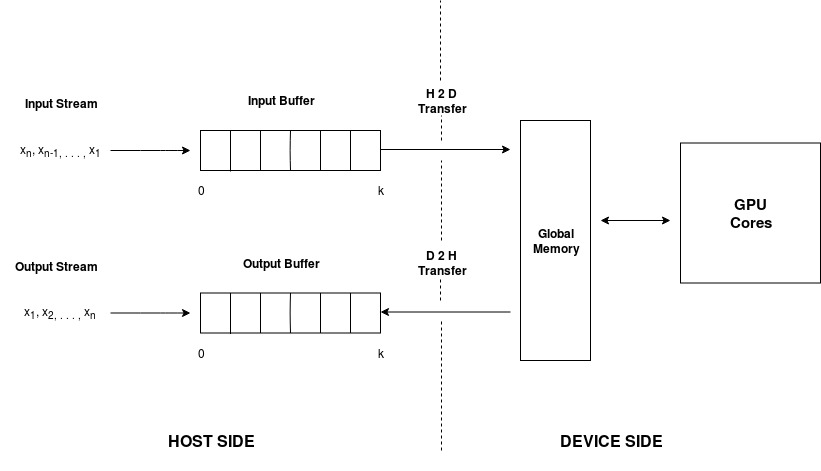
\includegraphics[width=\linewidth]{images/H2D.jpg}
		\caption{Here we have a general and broad graphical representation of our idea on how to fit a Farm parallel pattern on GPU architecture.}
		\label{fig:H2D}
	\end{figure}
	
	This behavior is illustrated graphically in Figure \ref{fig:H2D}. Here we can see our input stream, every \(k\) items we transfer them to Global memory of GPU; items will be spread all over warps in a way such that on every item will be applied all calculations, specified inside kernel code.\\
	

	From that figure it may seems we're sending only \(k\) items at time to/from GPU;but, assuming \(k\) items as a single item, this would correspond almost on a farm with one worker, processing one item per time. And this isn't surely what we want.\\
	And this is here where CUDA Streams \footnote{Don't confuse input/output stream in Farm parallel pattern with CUDA Streams.\\ These are two completely different notions: the first refers to the parallel pattern behavior of input/output data, the last refers to special CUDA commands (shown in \hyperref[subs:streams]{Section 2.3.3})} come into play.\\
	
	
	
		
		
		%\newpage \vspace*{\fill} 
		%\begin{sidewaysfigure}
		\begin{figure}
			%	\hspace*{-2cm}  
			\vspace{-2cm}
			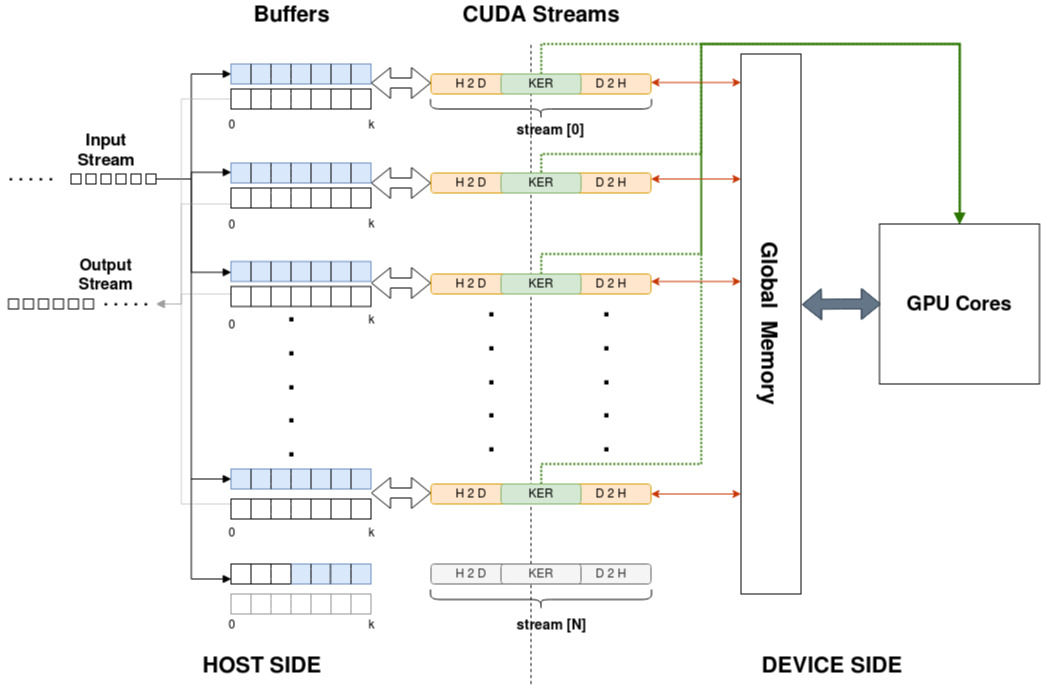
\includegraphics[scale=0.62,angle=-90]{images/overallLogic.jpg}
			\caption{Here we have a general and broad graphical representation of our idea on how to fit a Farm parallel pattern on GPU architecture.}
			\label{fig:overallLogic}
			

		\end{figure}
		
		
		%\begin{figure}
		%	\left
		%	\vspace{-4cm}
		%	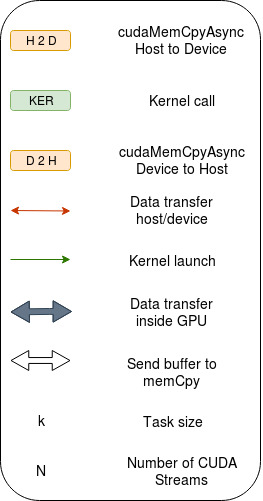
\includegraphics[scale=0.8]{images/logicLegenda.jpg}
		%	\caption{Legenda about Figure \ref{fig:overallLogic}.}
		%	\label{fig:logLegend}
		%\end{figure}
				
		
		\begin{wrapfigure}{r}{0.5\textwidth}
			%\begin{center}
			\raggedleft
				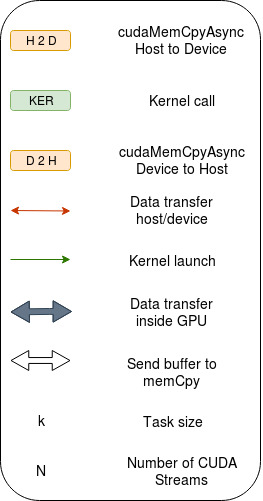
\includegraphics[width=0.48\textwidth]{images/logicLegenda.jpg}
			%\end{center}
			\caption{Legenda about Figure \ref{fig:overallLogic}.}
		\end{wrapfigure}
				
				
		%\end{sidewaysfigure}
		%\vspace*{\fill} \newpage
	
	
	We've based the use of CUDA Streams on the following ideas:
	\begin{enumerate}
		\item we have as many streams as Streaming Multiprocessors \footnote{Again CUDA Streams are a different concepts with respect to Streaming Multiprocessors. The first are a set of commands, the last are physical processing units.\\} and, at any given time, each of them hopefully issues a data transfer or a kernel executions;
		\item when we arrive at the point where all stream, sooner or later, issues a kernel launch (a maximum speed in a sense) ideally we expect that each kernel execution is taken over by a certain multiprocessor;
		\item obviously each kernel execution configuration should be well tuned, in order to take advantage of the maximum of resources in a multiprocessor. 
	\end{enumerate}
	
	All of those parameters have been established at first with some reasoning and assumptions on NVIDIA GPUs nature, later we moved on experimental proves \footnote{We'll see in next section more informations about Tunings.}. Measures and other estimation lead us to consider specific values for those variable parameters.\\
	Bringing all pieces together we can summarize all project logic in Figure \ref{fig:overallLogic}.
	Putting down in words that schema:
	
	\begin{itemize}
		\item we have \(N\) CUDA streams, where \(N\) is the number of Streaming Multiprocessors;
		\item as input stream items arrive, we let them fill buffers;
		
		\item in a Round-Robin fashion we spread buffers all over the CUDA streams as follows:
		\begin{enumerate}
			\item as soon as the \(i^{th}\) buffer is full, it's asynchronously sent on \texttt{stream [i]} to the GPU \\ 
			\texttt{ cudaMemcpyAsync( devBuffer, hostBuffer, bytes, \\ \tab \tab \tab \tab cudaMemcpyHostToDevice, stream[i]);}
			
			\item soon after we call the kernel, on the \texttt{stream [i]}, to make desired computations on that buffer;
			
			\item then, asynchronously again, we bring back results to host side \\
			\texttt{ cudaMemcpyAsync( devBuffer, hostBuffer, bytes,\\ \tab \tab \tab \tab
			 cudaMemcpyHostToDevice, stream[i]);}
			\item hopefully a Streaming Multiprocessor or a part, is made busy;
		\end{enumerate}
		
		
	\end{itemize}
	
	Initially only few cores will be really busy, but as soon as the buffers and streams get full, the pressure on the GPU will increase, so we expected that workload should be enough to almost fill all of Streaming multiprocessors.
	For us this means that we tried to have the maximum number of active threads inside each SM, having to do some work.\\
	



		\begin{figure}
			%	\hspace*{-2cm}  
			%\vspace{-2cm}
			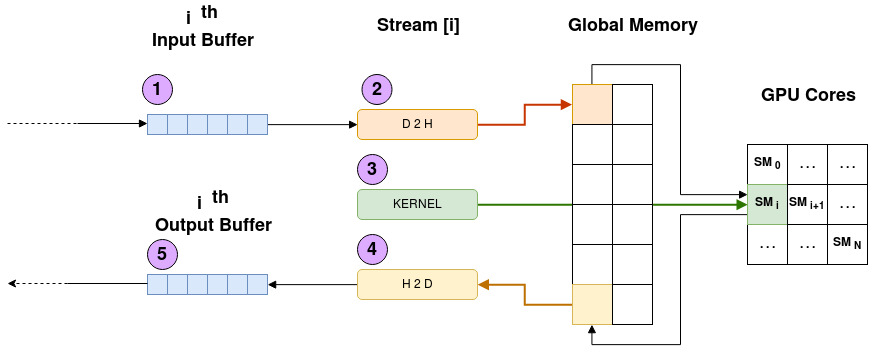
\includegraphics[scale=0.56]{images/singleStream.jpg}
			\caption{Here we can see what exactly happen in a certain CUDA Stream. Light violet numbered labels shows the order in which commands are issued by host to a certain stream.}
			\label{fig:singleStream}		
			
		\end{figure}
		
		
		
		To put a magnifying glass upon Figure \ref{fig:overallLogic} and to take a closer look to what we just said, check Figure  \ref{fig:singleStream}.\\
		From that we can see the order in which we issue command in a stream, and this will be the order in which they will be issued to device side too, for that stream.
		But we take advantage of the fact that we can overlap data transfer and/or kernel execution in a \texttt{stream [i]} with the ones in a \texttt{stream [k]} or \texttt{stream [j]} (for some \(k,j \in [0,N-1], for N =\# SMs\)).
		Note that in the Figure \ref{fig:singleStream}, we represented a kernel execution as fully occupying an entire SM; in reality it's not exactly how it goes.
		We'll see how we managed and tried out the Streaming Multiprocessors \textit{occupancy} in \hyperref[chap:experim]{Chapter 5}. \\
		
		So essentially if all of our reasoning and theories are right, we would expect that we can have an improvement, on completion time, roughly in the order of SMs number with respect to the \textit{classical approach} \footnote{By "classical approach" we mean to transfer data and execute kernels without any type of overlapping.\\ This is equivalent to send input, wait for data transfer completion on host, call kernel, send data back to host, only when they are a ready result and they are then transferred back to the waiting host.}.
		This similarly means that if, for example, we have 3 CUDA Stream we would expect to take an advantage on only at most 3 SMs (at peak work flow), so this should give us an improvement in completion time of at most 3 times, compared to classical approach.\\
		
		 
\section{Tunings}
	
	We followed for first some important best practices to obtain some good tunings:

	\begin{itemize}
		\item The effect of execution configuration on performance for a given kernel call generally
		depends on the kernel code, so experimentation is recommended and in fact we done this;
		\item The number of threads per block should be chosen as a multiple of the warp size (generally equal to 32 threads) to
		avoid wasting computing resources with under-populated warps as much as possible;
		\item we exploited \textbf{\textit{Occupancy Calculator}} both in spreadsheet and API functions formats \footnote{Those tools are included in CUDA Toolkit, they assist programmers in choosing thread block size based on kernel behavior, register and shared memory requirements.}, \cite{cudaguide}.
		 
	\end{itemize}

	Given those initial guidelines, it's important to highlight what are variable parameters in Figure \ref{fig:H2D}, on which the tuning was made:
	\begin{itemize}
		\item the number of Streams;
		\item the number of threads per block (block size);
		\item the number of blocks (grid size);
		\item the buffer dimension.
	\end{itemize}
	
	After lots of attempts and experiments, for each kernel type, we extrapolated best suitable values \footnote{Check \hyperref[chap:experim]{Chapter 5} to see all main values and their respective performances }.\\\\
	


\section{CPU/GPU Scheduling}
In addition to the main logic of our project we introduced another branch of study.\\
In particular, we extended the Farm parallel pattern on GPGPU introducing a sort of \textit{\textbf{CPU/GPU Scheduler}}.
This consist in an implementation that, given an initial work percentage, it gradually and experimentally tunes those percentages to balance jobs.
In particular, the scheduler adjusts the dimensions of data chunks directed to CPU or GPU on the basis of previous measured completion times of both processors.\\
Clearly, starting from a user provided percentage, measured times are used to recompute percentages (and thus chunks dimension). So, in a finite number of algorithm steps, the two portion size will stabilize around two values.\\
This allow us to let host and device cooperate to apply same computations, but with different workloads. Clearly the main idea is to let GPU have a greater workload with respect to the one for CPU, so that  latter can be lighten from doing the entire computations; at the same time, having a good occupancy on GPU, we can gain a speedup compared to letting only one of the two processors doing all the work.\\


